\documentclass{beamer}
\beamertemplatenavigationsymbolsempty
\usetheme{Madrid}
\usepackage{graphicx, hyperref, amsmath, animate, tabularx}
\usecolortheme{beaver}
\usefonttheme{professionalfonts}
\graphicspath{{./Figures/}}

\usepackage[backend=bibtex, style=verbose, sorting=none, autocite=footnote]{biblatex}
\addbibresource{ref.bib}
\renewcommand*{\bibfont}{\scriptsize}
\setbeamerfont{footnote}{size=\tiny}

\title[DS 691: RnD Project]{Localizing Text Across Domains Using RARR Attribution Technique}
\author[Soumen Mondal]{Soumen Kumar Mondal\\\texttt{23m2157@iitb.ac.in}}
\institute[IIT Bombay]{Guide: Prof. Preethi Jyothi\\\;\\Indian Institute of Technology Bombay}
\date{May 8, 2024}

\begin{document}
	% Title page frame
	\begin{frame}
		\titlepage
	\end{frame}
	
	\begin{frame}{Problem Statement}
		\begin{block}{\scriptsize What is Text Localization?}\scriptsize
			Text localization and adaptation across domains involve modifying textual content to suit different cultural and geographical contexts while maintaining the original message's context, style and intent.
		\end{block}
		\begin{block}{\scriptsize Problem of Text Localization}\scriptsize
			\begin{figure}
				\centering
				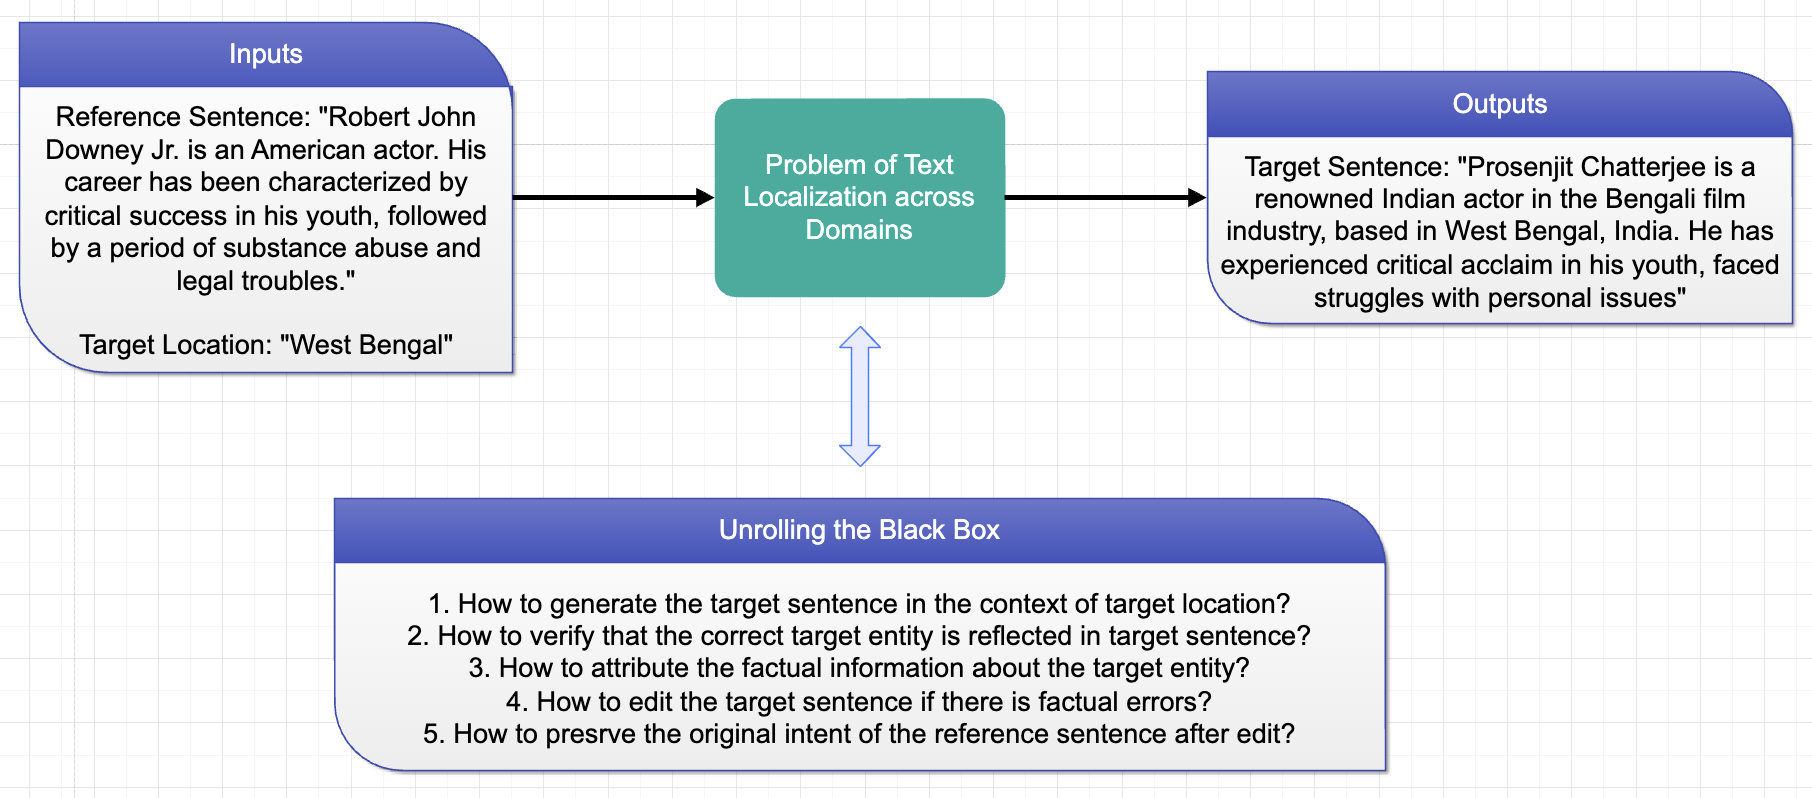
\includegraphics[width=0.95\textwidth]{problem-statement.png}
			\end{figure}
		\end{block}
	\end{frame}
	
	\begin{frame}{RARR System}
		\begin{columns}
			\column{0.3\textwidth}
			\begin{block}{\scriptsize What is RARR?}\scriptsize
				The Retrofit Attribution using Research and Revision (RARR) model is an approach designed to use for text attribution, ensuring that the content does not contain any factual misinformation while preserving the intent of the original text.
			\end{block}
			\column{0.6\textwidth}
			\begin{block}{\scriptsize Overview of Original RARR System\footnotemark}\scriptsize
				\begin{figure}
					\centering
					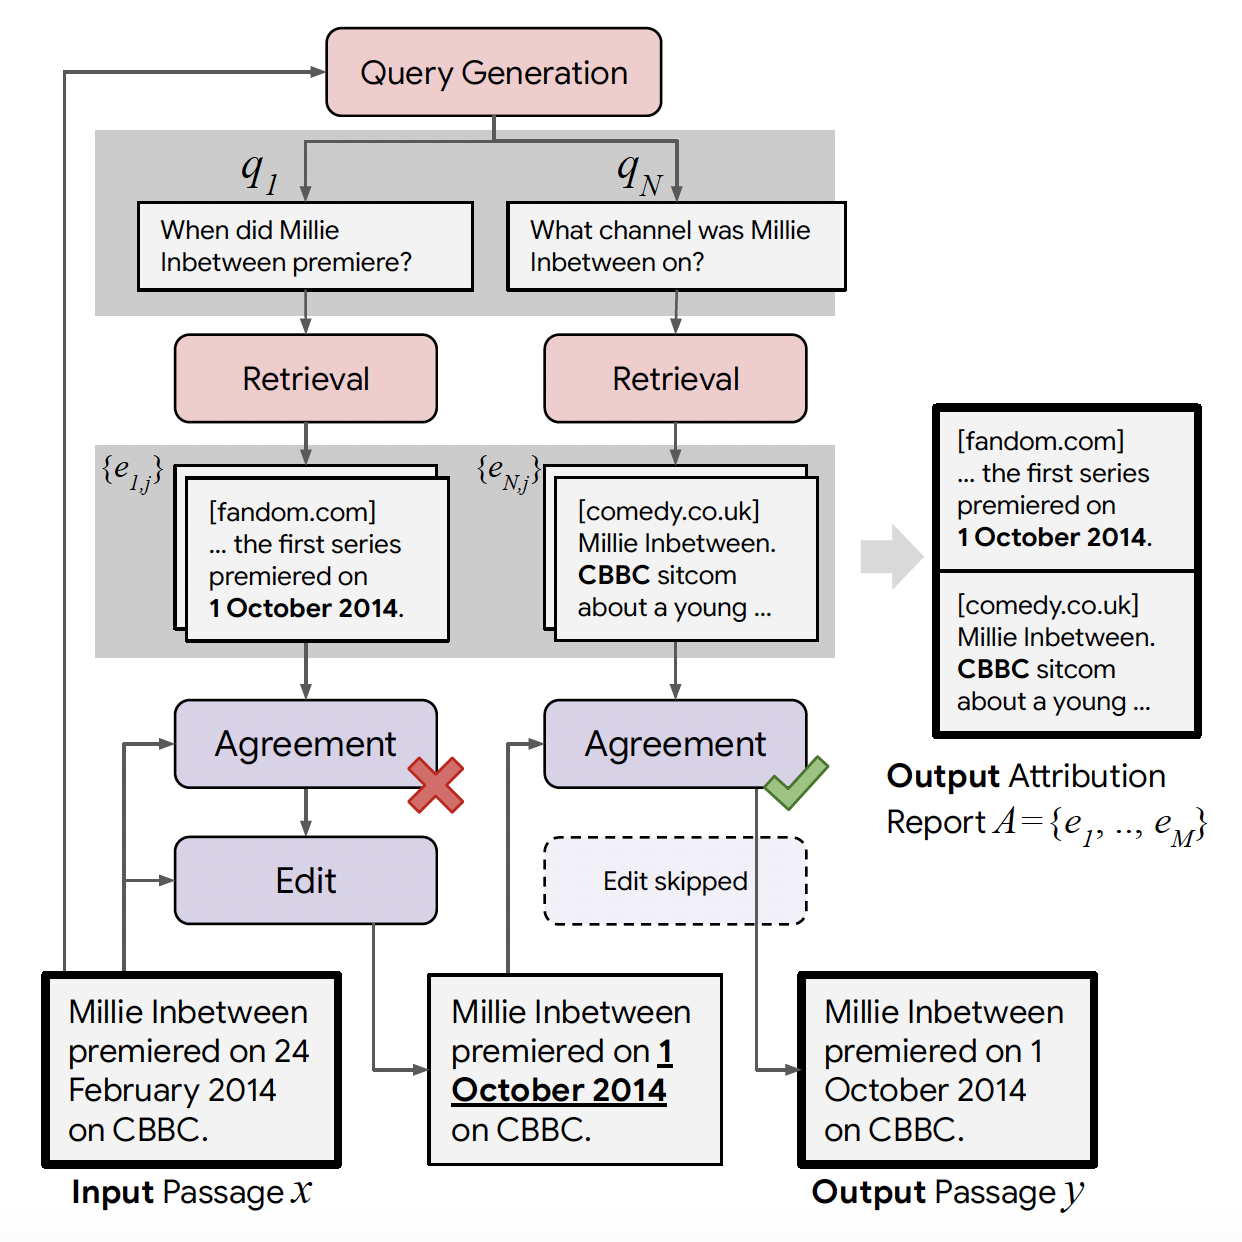
\includegraphics[width=0.85\textwidth]{rarr.png}
				\end{figure}
			\end{block}
		\end{columns}\footcitetext{gao2023rarr}
	\end{frame}
	
	\begin{frame}{Stage 1: Question Generation}
		\begin{block}{\scriptsize Workflow of Stage 1}\scriptsize
			\begin{figure}
				\centering
				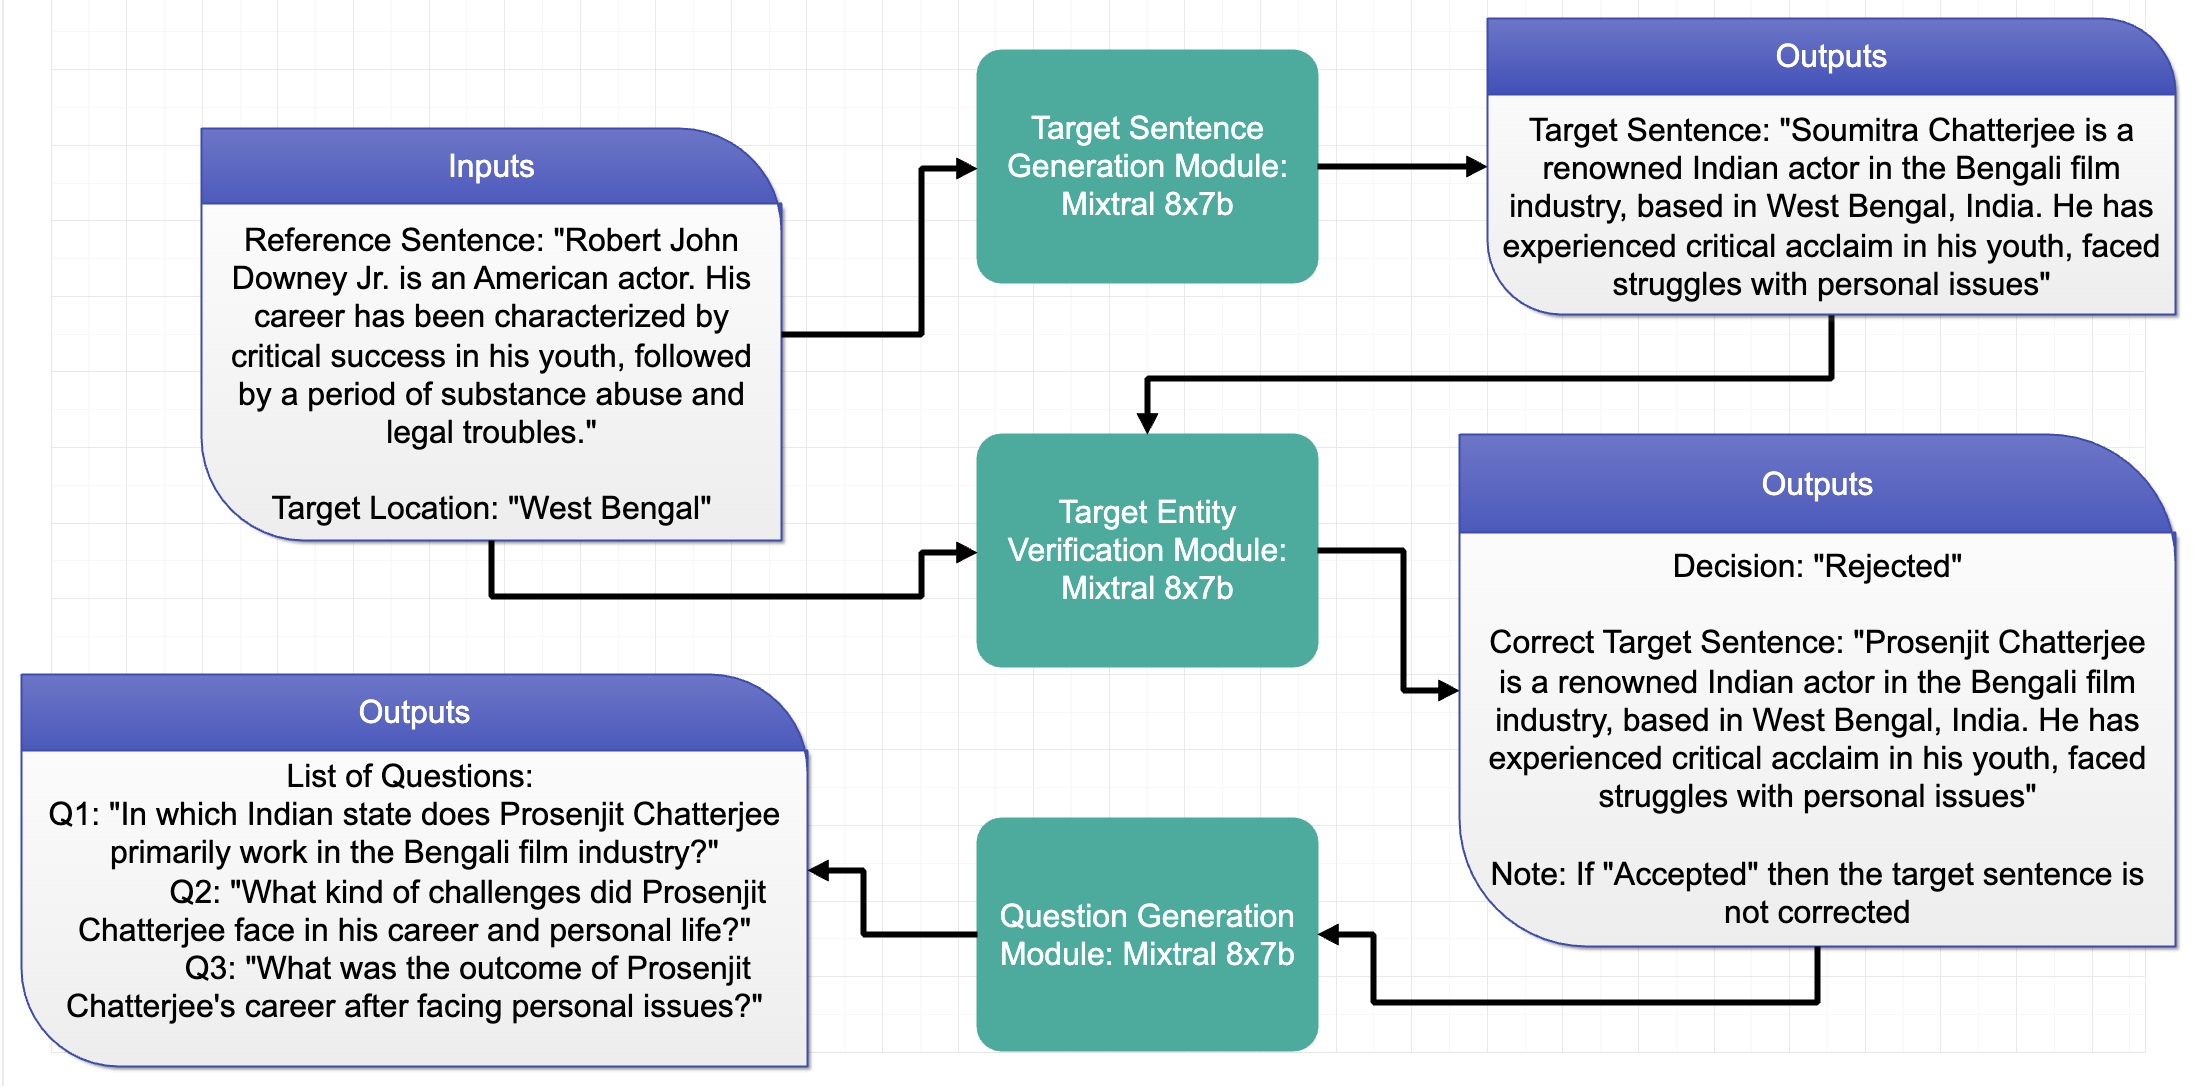
\includegraphics[width=0.7\textwidth]{module123.png}
			\end{figure}
		\end{block}
		\begin{block}{\scriptsize Critical Analysis of Stage 1}\scriptsize
			\begin{itemize}
				\item Mixtral 8x7b model\footnotemark output is not deterministic when the reference sentence contains facts such as date, time, place of incidents.
				\item Target Entity Verification Module can be checked by GPT 3.5 or 4 for effective results.
			\end{itemize}
		\end{block}
		\footcitetext{jiang2024mixtral}
	\end{frame}
	
	\begin{frame}{Stage 2: Evidence Retrieval}
		\begin{block}{\scriptsize Workflow of Stage 2}\scriptsize
			\begin{figure}
				\centering
				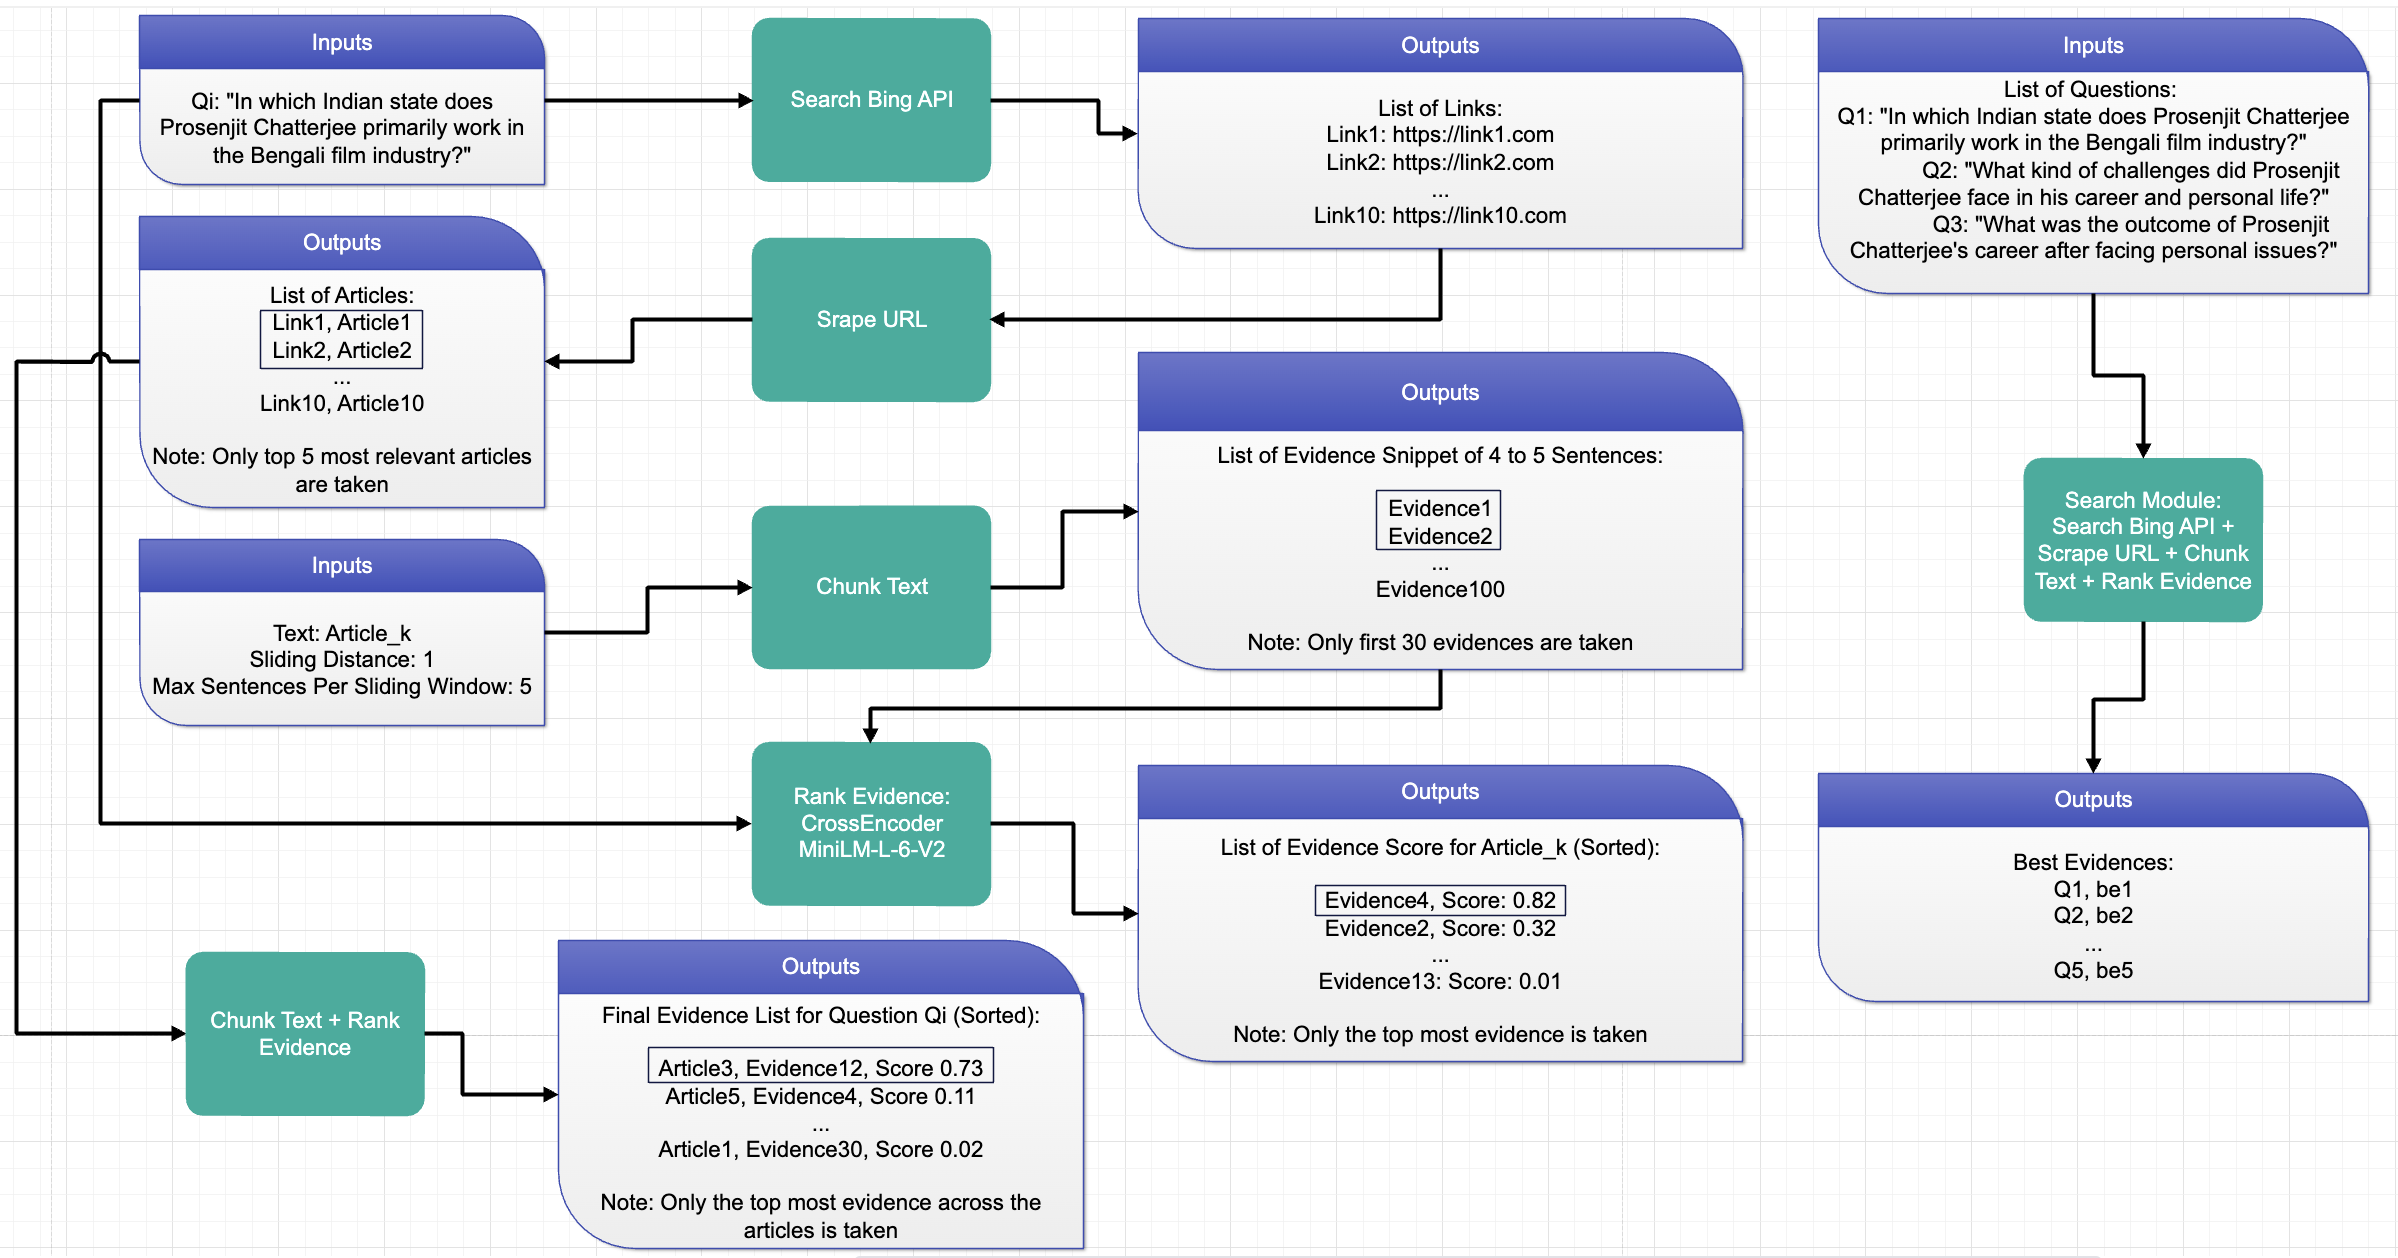
\includegraphics[width=0.775\textwidth]{module4.png}
			\end{figure}
		\end{block}
		\begin{block}{\scriptsize Critical Analysis of Stage 2}\scriptsize
			\begin{itemize}
				\item Bing is unable to retrieve the relevant links if the target location is absent in the question.
				\item The first 30 passages from each article may not contain the relevant information.
				\item Instead of CrossEncoder, different embedding model can be used.
			\end{itemize}
		\end{block}
	\end{frame}
	
	\begin{frame}{Stage 3: Attribution}
		\begin{block}{\scriptsize Workflow of Stage 3}\scriptsize
			\begin{figure}
				\centering
				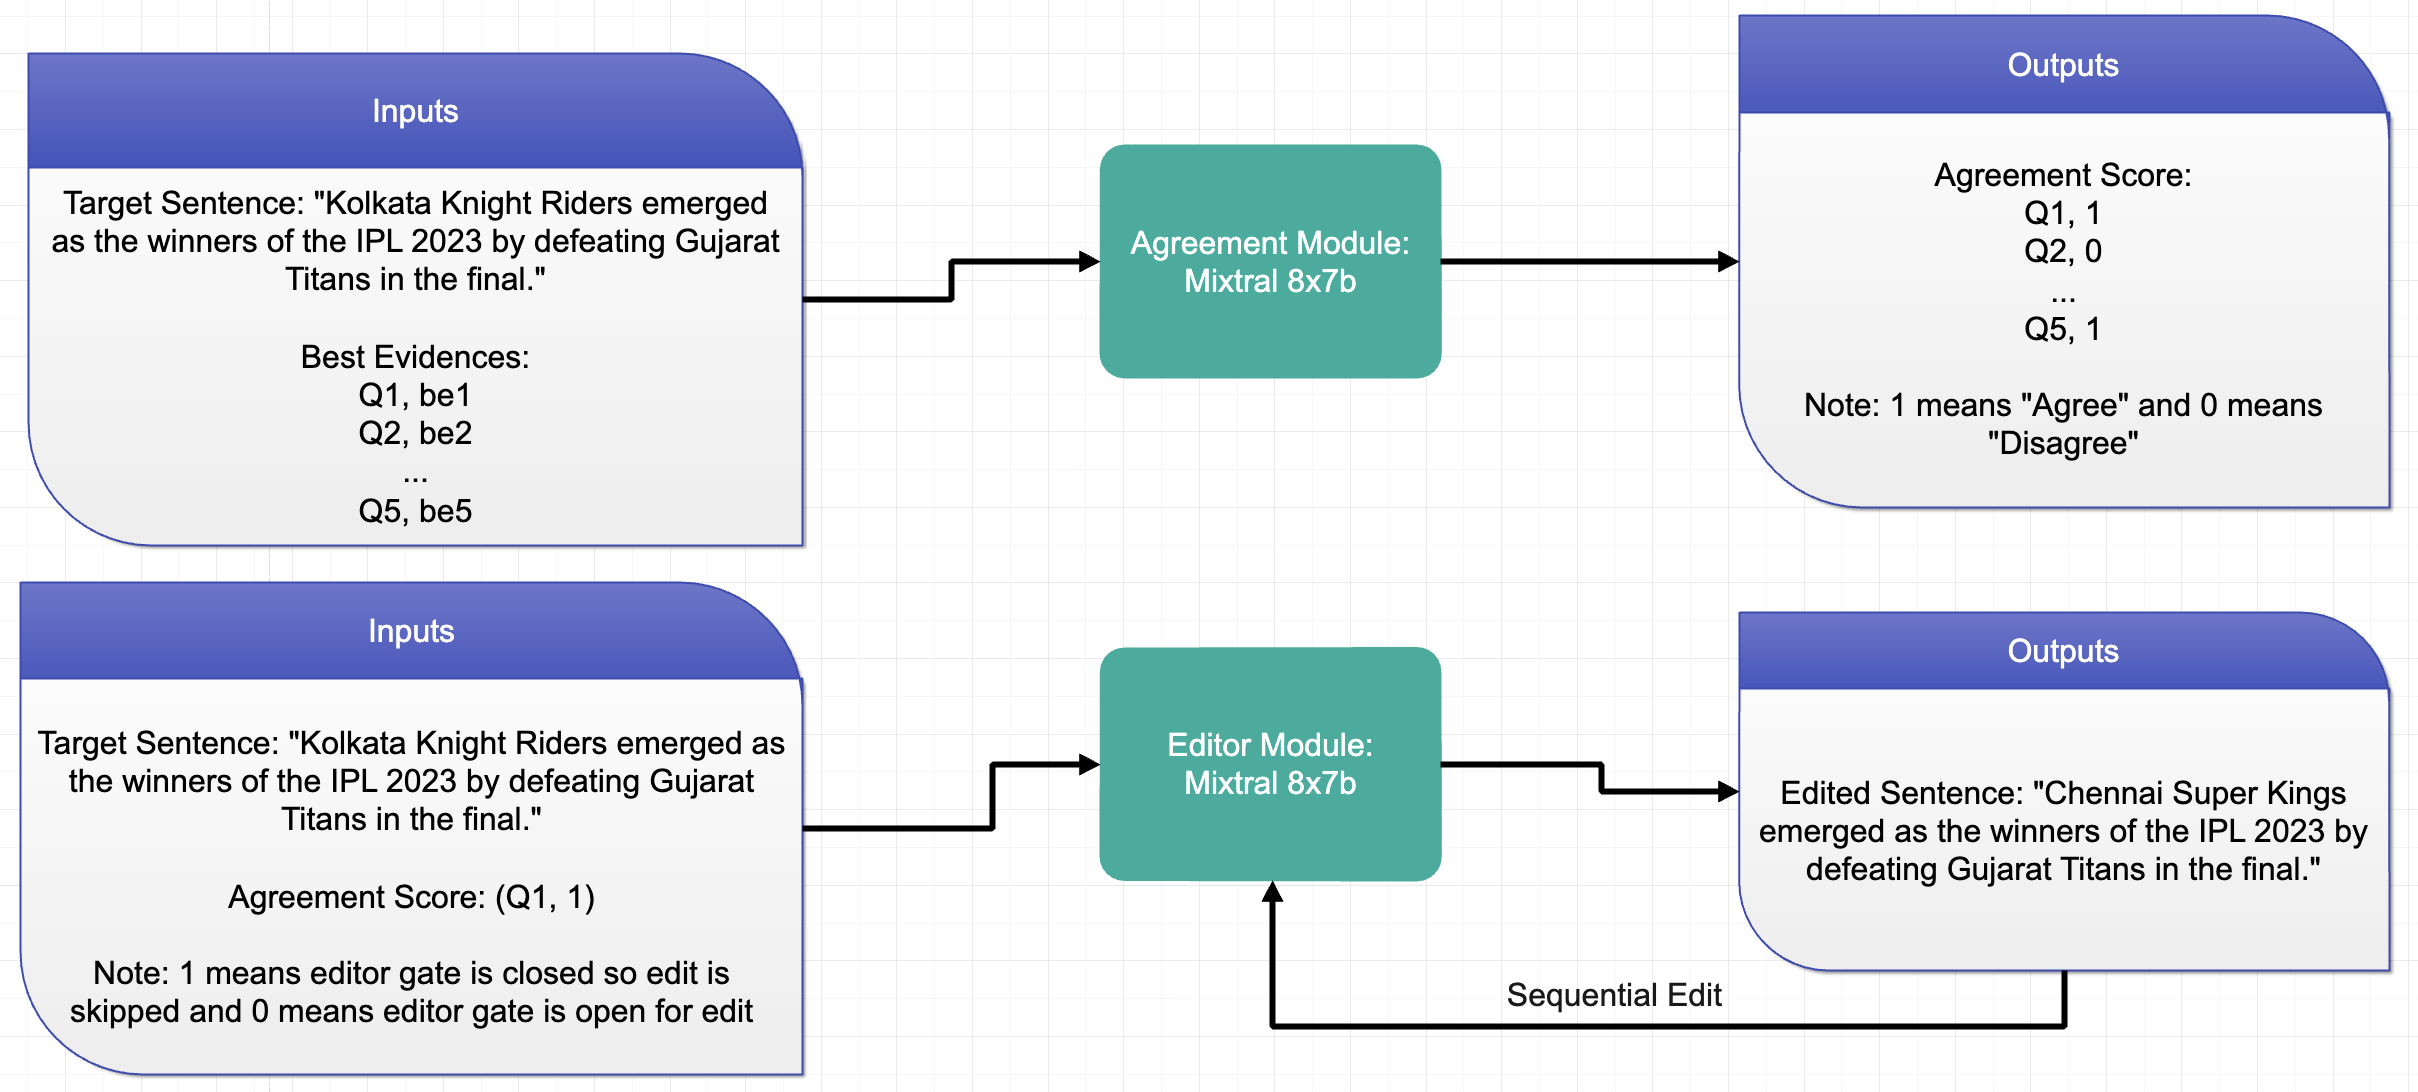
\includegraphics[width=0.8\textwidth]{module56.png}
			\end{figure}
		\end{block}
		\begin{block}{\scriptsize Critical Analysis of Stage 3}\scriptsize
			\begin{itemize}
				\item Sequential editing increases the length of the output target sentence which fails to preserve the style and intent of original target sentence.
				\item RARR helps in attribution but fails to outperform Mixtral 8x7b localize text based on target location.
			\end{itemize}
		\end{block}
	\end{frame}
	
	\begin{frame}{Evaluation Dataset}
		\begin{block}{\scriptsize Sample Example of Dataset}\scriptsize
			\begin{table}
				\centering
				\begin{tabularx}{\textwidth}{XXXX}
					\hline
					\textbf{Category, Reference and Target Location} & \textbf{Reference Sentence} & \textbf{Target Sentence} & \textbf{Common Questions} \\ \hline
					Actor/Actress, US, Kerala & Dwayne Douglas Johnson, also known by his ring name the Rock, is an American actor and professional wrestler currently signed to WWE. & Mohanlal, also known by his pet name "Lalettan", is an Indian actor and producer, currently working in the Malayalam film industry. & (i) Can you give an example of an actor who professionally holds another title as well?
					(ii) Can you provide the name of an actor who is well-known in the entertainment industry by another name? \\
					\hline
				\end{tabularx}
			\end{table}
		\end{block}
		\begin{block}{\scriptsize Critical Analysis of Dataset}\scriptsize
			\begin{itemize}
				\item There could be multiple answer to the common question in the context of target location.
				\item Human annotation is needed to improve the quality of common questions.
			\end{itemize}
		\end{block}
	\end{frame}
	
	\begin{frame}{Common Question Evaluation Metric}
		\begin{block}{\scriptsize Definition}\scriptsize
			\begin{itemize}
				\item We use few shot prompting with GPT 3.5 to check if the answer to the common question in the context of target location is contained in the target sentence. 
				\item $S^i$: A target sentence (RARR edited target sentence output or Mixtral 8x7b output.
				\item $m_i$: The number of generated questions.
				\item  $\{q_j^i\}_{j=1}^{m_i}$: The list of generated questions.
				\item $\{A_j^i\}_{j=1}^{m_i}$: The binary score provided by GPT 3.5.
				\item $N$: The total number of sentences.
				\item $Q = \sum_{i=1}^N m_i$: Total number of questions over this $N$ sentences.
			\end{itemize}

			\begin{equation}
				C_{CQ} = \frac{1}{Q} \sum_{i=1}^{N} \sum_{j=1}^{m_i} A_j^i
			\end{equation}
		\end{block}
		\begin{block}{\scriptsize Interpretation}\scriptsize
			\begin{itemize}
				\item A higher score $C_{CQ}$ indicates that the model is more effective at editing target sentences that contain accurate and relevant answers to the posed questions.
				\item This measure directly reflects the model's capability to understand and adapt the context of the reference location to the target location.
			\end{itemize}
		\end{block}
	\end{frame}
	
	\begin{frame}{Results and Discussion}
		\begin{block}{\scriptsize Attribution Results by RARR}\scriptsize
			\begin{figure}
				\centering
				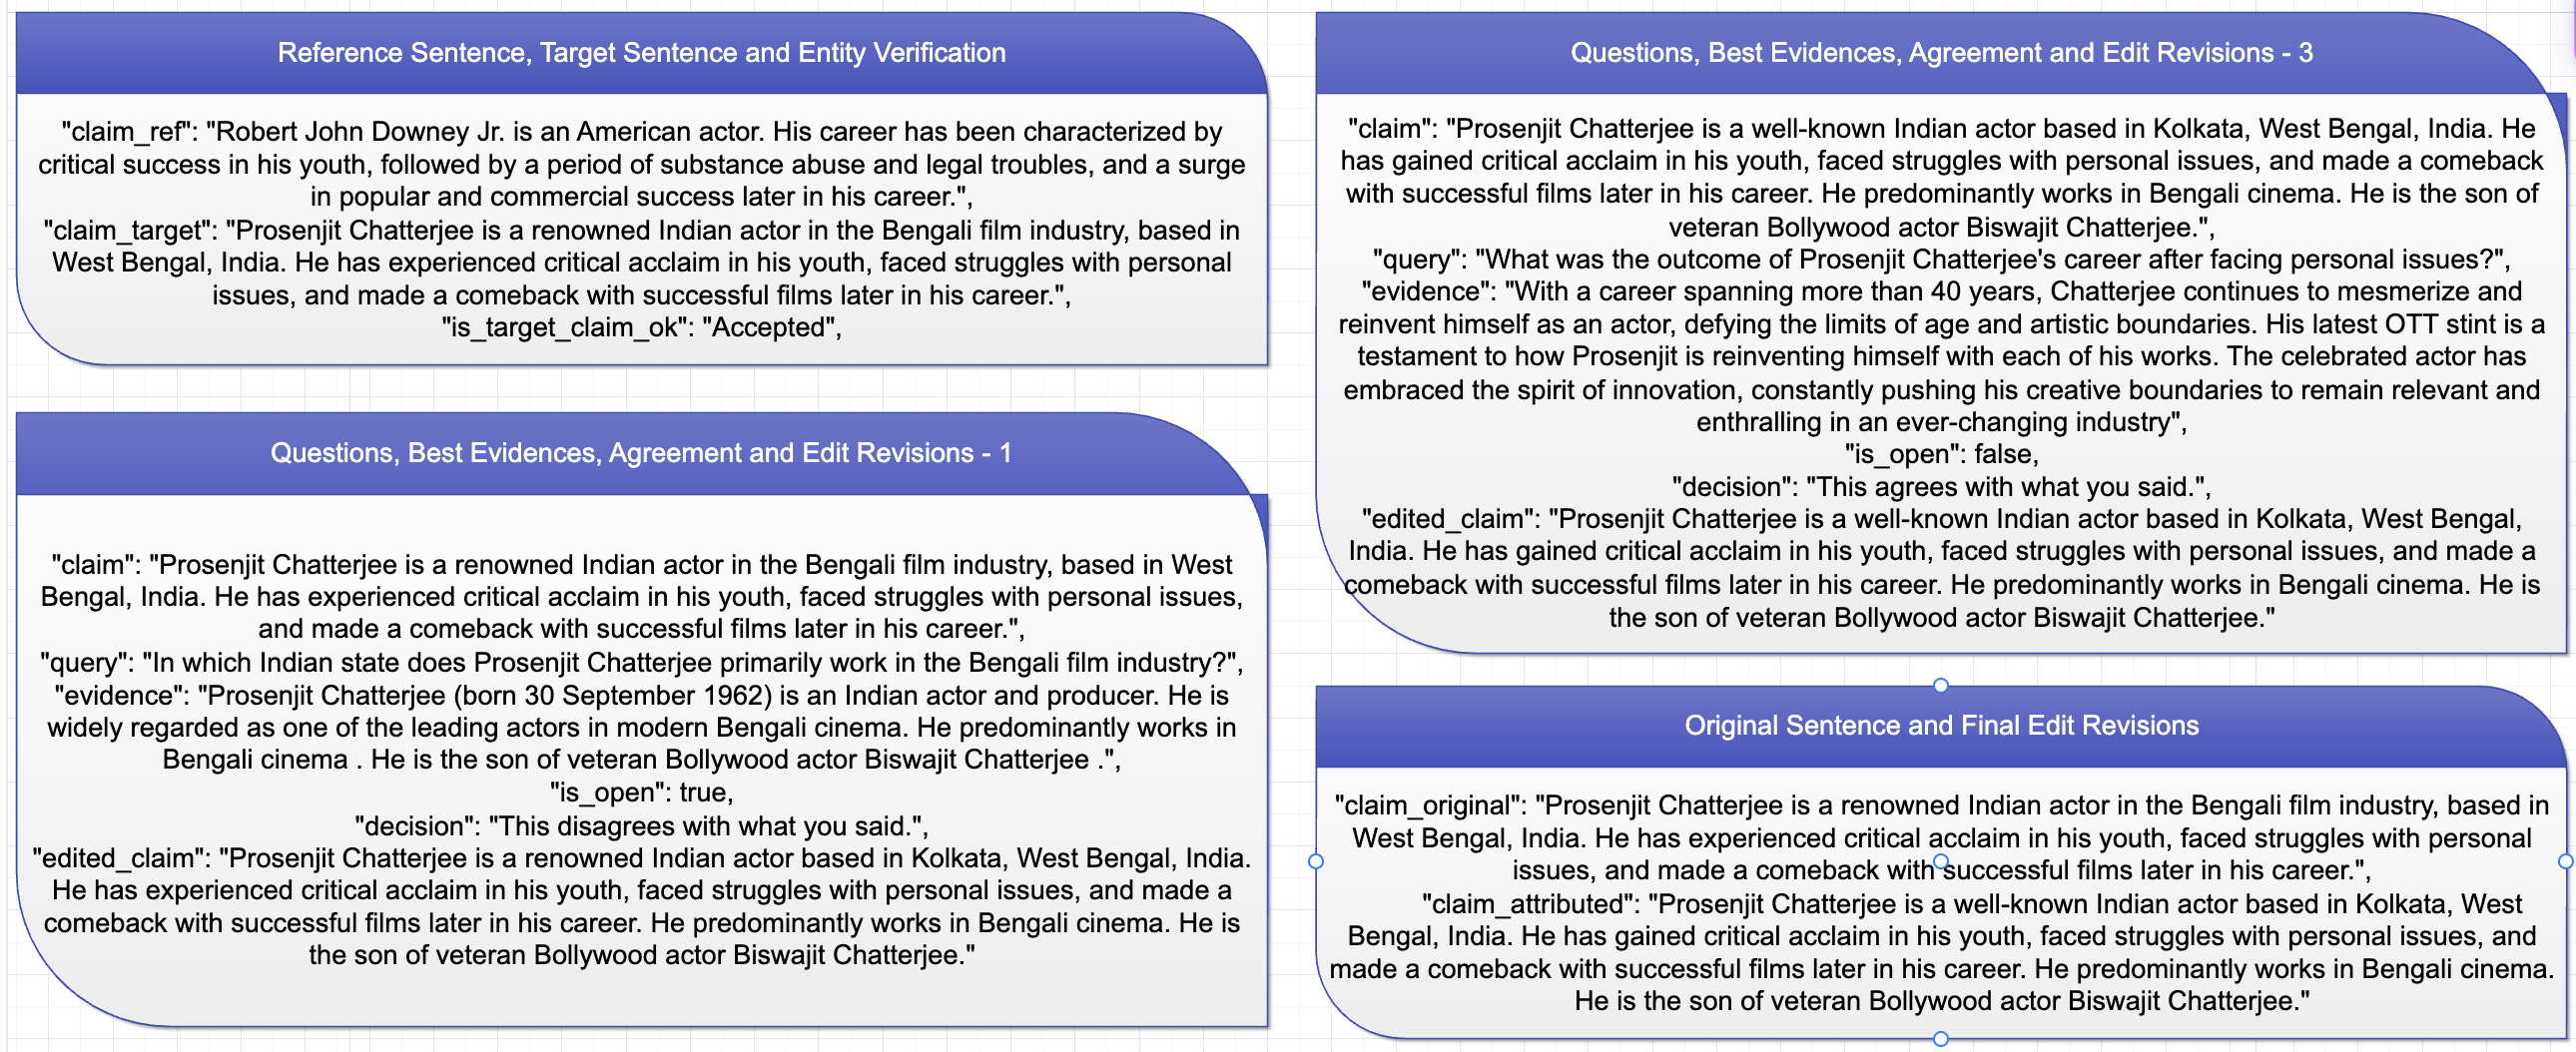
\includegraphics[width=\textwidth]{result.png}
			\end{figure}
		\end{block}
		\begin{block}{\scriptsize Key Findings} \scriptsize
			\begin{itemize}
				\item Sequential edit increases the length of the target sentence. Furthermore, it changes the style and intent of original sentence.
			\end{itemize}
		\end{block}
	\end{frame}
	
	\begin{frame}{Results and Discussion [Contd.]}
		\begin{block}{\scriptsize Localization Results}\scriptsize
			\begin{table}
				\centering
				\begin{tabularx}{\textwidth}{XX}
					\hline 
					\textbf{Model} & \textbf{Common Question Evaluation Metric $C_{CQ}$}  \\ \hline
					RARR Baseline & 0.5836 \\
					RARR Single Edit &0.6411 \\
					Mixtral 8x7b & 0.6439 \\
					\hline
				\end{tabularx}
			\end{table}
		\end{block}
		\begin{block}{\scriptsize Discussion}\scriptsize
			\begin{itemize}
				\item The results are averaged over 200 samples with 3 instances of target sentence generation.
				\item The results show that the Mixtral 8x7b outperforms RARR model in the common question evaluation metric indicating the improvement required in the RARR baseline model. 
				\item However, this metric does not capture the attribution quality of the RARR. 
				\item It has also been observed that the RARR model is better than Mixtral 8x7b in terms of attribution but cannot outperform Mixtral 8x7b in text localization.
				\item Ablation study shows that the single edit is effective for the common question metric than the sequential edit.
				\item Changing the number of passages and embedding type do not affect the common question metric.
			\end{itemize}
		\end{block}
	\end{frame}
	
	\begin{frame}{Conclusion and Future Work}
		\begin{block}{\scriptsize Conclusion}\scriptsize
			\begin{itemize}
				\item This study has explored the effectiveness of the RARR model in the field of text localization and adaptation across diverse geographical domains. 
				\item The evaluation of the model using a comprehensive dataset and a set of common questions has revealed that the RARR model performs better in attribution of factual information but cannot beat Mixtral 8x7b for text localization.
			\end{itemize}
		\end{block}
		\begin{block}{\scriptsize Future Works}\scriptsize
			\begin{itemize}
				\item \textbf{Improving Model Robustness:} Future iterations of the RARR model will focus on enhancing the search module of RARR model indicating the use of Retrieval Augmented Models.
				
				\item \textbf{Enhanced Evaluation Metrics:} The metric currently is solely based on GPT 3.5 model. However, we can use GPT 4 model\footnotemark for the evaluation purpose.
			\end{itemize}
		\end{block}\footcitetext{openai2024gpt4}
	\end{frame}
	
	\section{References}
	\begin{frame}{References}
		\begin{block}{}\scriptsize
			\printbibliography
		\end{block}
	\end{frame}
	
	\begin{frame}{}
		\centering \Huge
		\emph{Thank You!}
	\end{frame}
	
\end{document}